\documentclass[twocolumn,astrosymb,twocolappendix]{aastex631}

%% The default is a single spaced, 10 point font, single spaced article.
%% There are 5 other style options available via an optional argument. They
%% can be invoked like this:
%%
%% \documentclass[arguments]{aastex631}
%% 
%% where the layout options are:
%%
%%  twocolumn   : two text columns, 10 point font, single spaced article.
%%                This is the most compact and represent the final published
%%                derived PDF copy of the accepted manuscript from the publisher
%%  manuscript  : one text column, 12 point font, double spaced article.
%%  preprint    : one text column, 12 point font, single spaced article.  
%%  preprint2   : two text columns, 12 point font, single spaced article.
%%  modern      : a stylish, single text column, 12 point font, article with
%% 		  wider left and right margins. This uses the Daniel
%% 		  Foreman-Mackey and David Hogg design.
%%  RNAAS       : Supresses an abstract. Originally for RNAAS manuscripts 
%%                but now that abstracts are required this is obsolete for
%%                AAS Journals. Authors might need it for other reasons. DO NOT
%%                use \begin{abstract} and \end{abstract} with this style.
%%
%% Note that you can submit to the AAS Journals in any of these 6 styles.
%%
%% There are other optional arguments one can invoke to allow other stylistic
%% actions. The available options are:
%%
%%   astrosymb    : Loads Astrosymb font and define \astrocommands. 
%%   tighten      : Makes baselineskip slightly smaller, only works with 
%%                  the twocolumn substyle.
%%   times        : uses times font instead of the default
%%   linenumbers  : turn on lineno package.
%%   trackchanges : required to see the revision mark up and print its output
%%   longauthor   : Do not use the more compressed footnote style (default) for 
%%                  the author/collaboration/affiliations. Instead print all
%%                  affiliation information after each name. Creates a much 
%%                  longer author list but may be desirable for short 
%%                  author papers.
%% twocolappendix : make 2 column appendix.
%%   anonymous    : Do not show the authors, affiliations and acknowledgments 
%%                  for dual anonymous review.
%%
%% these can be used in any combination, e.g.
%%
%% \documentclass[twocolumn,linenumbers,trackchanges]{aastex631}
%%
%% AASTeX v6.* now includes \hyperref support. While we have built in specific
%% defaults into the classfile you can manually override them with the
%% \hypersetup command. For example,
%%
%% \hypersetup{linkcolor=red,citecolor=green,filecolor=cyan,urlcolor=magenta}
%%
%% will change the color of the internal links to red, the links to the
%% bibliography to green, the file links to cyan, and the external links to
%% magenta. Additional information on \hyperref options can be found here:
%% https://www.tug.org/applications/hyperref/manual.html#x1-40003
%%
%% Note that in v6.3 "bookmarks" has been changed to "true" in hyperref
%% to improve the accessibility of the compiled pdf file.
%%
%% If you want to create your own macros, you can do so
%% using \newcommand. Your macros should appear before
%% the \begin{document} command.
%%
\newcommand{\vdag}{(v)^\dagger}
\newcommand\aastex{AAS\TeX}
\newcommand\latex{La\TeX}
\newcommand{\sbunit}{mag~arcsec$^{-2}$}

\newcommand{\code}[1]{\textbf{\texttt{#1}}}
\newcommand{\sersic}{S\'ersic}
\usepackage{CJKutf8}
\usepackage{bm}
\usepackage{appendix}
\usepackage{amsmath,amssymb}

%% Reintroduced the \received and \accepted commands from AASTeX v5.2
\received{\today}
\revised{\today}
\accepted{\today}

\submitjournal{ApJ}

%% alias for citations
\defcitealias{Greco2018}{G18}

% \def\G18{\citetalias{Greco2018}}

\shorttitle{UDGs in MW analogs}
\shortauthors{Li et al.}
%%
%% You can add a light gray and diagonal water-mark to the first page 
%% with this command:
%% \watermark{text}
%% where "text", e.g. DRAFT, is the text to appear.  If the text is 
%% long you can control the water-mark size with:
%% \setwatermarkfontsize{dimension}
%% where dimension is any recognized LaTeX dimension, e.g. pt, in, etc.
%%
%%%%%%%%%%%%%%%%%%%%%%%%%%%%%%%%%%%%%%%%%%%%%%%%%%%%%%%%%%%%%%%%%%%%%%%%%%%%%%%%
\graphicspath{{./}{figures/}}
%% This is the end of the preamble.  Indicate the beginning of the
%% manuscript itself with \begin{document}.

\begin{document}
\begin{CJK*}{UTF8}{gbsn}

\title{Ultra Diffuse Galaxies associated with Milky-Way Analogs}

% \correspondingauthor{Jiaxuan Li}
\author[0000-0001-9592-4190]{Jiaxuan Li (李嘉轩)}
\affiliation{Department of Astrophysical Sciences, 4 Ivy Lane, Princeton University, Princeton, NJ 08544, USA}

\author[0000-0002-5612-3427]{Jenny E. Greene}
\affiliation{Department of Astrophysical Sciences, 4 Ivy Lane, Princeton University, Princeton, NJ 08544, USA}

\author[0000-0003-4970-2874]{Johnny Greco}
\affiliation{Department of Astrophysical Sciences, 4 Ivy Lane, Princeton University, Princeton, NJ 08544, USA}
\affiliation{Center for Cosmology and AstroParticle Physics (CCAPP), The Ohio State University, Columbus, OH 43210, USA}

\author[0000-0003-1385-7591]{Song Huang (黄崧)}
\affiliation{Department of Astrophysical Sciences, 4 Ivy Lane, Princeton University, Princeton, NJ 08544, USA}
\affiliation{Department of Astronomy and Tsinghua Center for Astrophysics, Tsinghua University, Beijing 100084, China}

\author[0000-0002-8873-5065]{Peter Melchior}
\affiliation{Department of Astrophysical Sciences, 4 Ivy Lane, Princeton University, Princeton, NJ 08544, USA}
\author[0000-0002-2704-5028]{Remy Joseph}
\affiliation{Department of Astrophysical Sciences, 4 Ivy Lane, Princeton University, Princeton, NJ 08544, USA}
\author[0000-0002-1841-2252]{Shany Danieli}
\affiliation{Department of Astrophysical Sciences, 4 Ivy Lane, Princeton University, Princeton, NJ 08544, USA}

%% I'd like to invite Shany?

%% Note that the \and command from previous versions of AASTeX is now
%% depreciated in this version as it is no longer necessary. AASTeX 
%% automatically takes care of all commas and "and"s between authors names.

%% AASTeX 6.31 has the new \collaboration and \nocollaboration commands to
%% provide the collaboration status of a group of authors. These commands 
%% can be used either before or after the list of corresponding authors. The
%% argument for \collaboration is the collaboration identifier. Authors are
%% encouraged to surround collaboration identifiers with ()s. The 
%% \nocollaboration command takes no argument and exists to indicate that
%% the nearby authors are not part of surrounding collaborations.

%% Mark off the abstract in the ``abstract'' environment. 
\begin{abstract}

\end{abstract}

\keywords{Low surface brightness galaxies (940), Dwarf galaxies (416), Galaxy properties (615), Galaxy abundances (574)}


\section{Introduction} \label{sec:intro}

In this work, we use the circularized effective radius $r_{\rm eff}$, defined as the $r_{\rm eff} = r_{\rm eff, sma} \sqrt{b/a}$, where $r_{\rm eff, sma}$ is the effective radius along the semi-major axis of the aligned elliptical isophotes, and $b/a$ is the axis ratio of the isophotes.

We adopt a $\Lambda$CDM cosmology from \citet{Planck15} with $\Omega_{\rm m}= 0.307$ and $H_0 = 67.7\ $km s$^{-1}$ Mpc$^{-1}$. We use the AB system \citep{Oke1983} for magnitudes. The stellar mass used in this work is based on a \citet{Chabrier2003} initial mass function.

\section{Data} \label{sec:data}
\subsection{Hyper Suprime-Camera data}
The Hyper Suprime-Camera Subaru Strategic Program Survey (\citealt{Aihara2018}; hereafter HSC survey)\footnote{\url{https://hsc-release.mtk.nao.ac.jp/doc/}} is an optical imaging survey using the 8.2-m Subaru telescope and the Hyper Suprime-Camera \citep{Miyazaki2012, Miyazaki2018}. The \texttt{Wide} layer is designed to cover $\sim 1000\ \rm{deg}^{2}$ of the sky in five broad bands ($grizy$), reaching a depth of $g=26.6$ mag, $r=26.2$ mag and $i=26.2$ mag ($5\sigma$ point source). HSC data are processed using \code{hscPipe}\footnote{\url{https://hsc.mtk.nao.ac.jp/pipedoc_e/}} \citep{Bosch2018}, which is a customized version of the Large Synoptic Survey Telescope (LSST) pipeline \citep{LSST-pipeline}\footnote{\url{https://pipelines.lsst.io/}}. 

In this work, we use the \code{Wide} layer data from Public Data Release 2 (PDR2, also known as \code{S18A}) of HSC \citealt{Aihara2018}. It covers $\sim 300\ \rm{deg}^2$ in all five bands, which is 1.5 times larger than the dataset analyzed in \citetalias{Greco2018}. One of the key improvements made in \code{S18A} is the sky background subtraction. Compared with previous data releases, \code{S18A} adopted a full focal plane sky subtraction algorithm to overcome the over-subtraction of local sky background around bright objects \citep{Aihara2018,Li2021}. The unprecedented depth and careful sky subtraction makes \code{S18A} an ideal dataset to search for low surface brightness galaxies. 

%HSC \code{S18A} also provides bitmasks indicating bad pixels, cosmic rays, edges of CCDs and pixels with source detection, helping us generate image masks when extracting surface brightness profiles (Section \ref{sec:hsc_methods}). In this paper, we use the \code{WIDE} layer data from \code{S18A} (\code{PDR2}). It covers $\sim 300$ deg$^2$ in all five bands. 

\subsection{NASA-Sloan Atlas}
We use the NASA-Sloan Atlas (NSA \footnote{\url{http://nsatlas.org}}, \citealt{Blanton2005,Blanton2011}) to select galaxies analogous to the Milky Way. NSA is a catalog of parameters of local galaxies derived from the Sloan Digital Sky Survey \citep[SDSS,][]{York2000}. We use the new version of NSA catalog (\code{v1\_0\_1}\footnote{\url{https://www.sdss.org/dr13/manga/manga-target-selection/nsa/}}) which contains about $640,000$ galaxies out to $z < 0.15$. It also includes elliptical Petrosian aperture photometry for galaxies, which is considered to be more reliable than the photometry used in older versions. In this paper, we use the stellar mass derived from the ellpitical Petrosian photometry using \code{kcorrect v4\_2}. The redshifts of galaxies in NSA come from several spectroscopic surveys, gas surveys, or direct distance measurements. 



\section{Methodology}
Given an overview of the steps here.

\subsection{Source Detection}\label{sec:detection}
\citetalias{Greco2018} performed a search for extended LSBGs in the first $\sim 200$ deg$^2$ of HSC survey. We continued the work in \citetalias{Greco2018} and extended the search to HSC \code{S18A} data which covers $\sim 300\ \rm{deg}^{2}$ and has much better sky subtraction compared to \code{S16A}. We follow the same philosophy of source detection as in \citetalias{Greco2018}, but make several updates to accommodate \code{S18A} data. Below we summarize the main steps of the search and emphasize the updates made to improve the overall completeness and purity. We refer interested readers to \citetalias{Greco2018} for more details. Our source detection pipeline \code{hugs}\footnote{\url{https://github.com/johnnygreco/hugs}} is also publically available.

\begin{enumerate}
    \item \textbf{Bright source removal}. Bright sources and their associated LSB lights can mimic objects of interest and obstruct effective detection of LSBGs. In this step, we replace pixels related to bright sources with sky noise. The bright sources and their diffuse lights are detected by applying a high thresholding and a low thresholding to the image. A diffuse light component is associated with a bright source if more than 15\% of its pixels are above the high threshold. In this way, we generate a footprint of bright sources in the image.
    
    Since the sky subtraction in \code{S18A} is significantly better than in previous data releases, LSB features are well conserved after subtracting the sky. Therefore, it makes more sense to set the thresholding based on surface brightness, instead of a certain sigma value above sky background (as in \citetalias{Greco2018}). We set the high threshold to $\mu_{\rm high} = 22\ \mathrm{mag\ arcsec^{-2}}$ to capture all bright sources above this surface brightness, and the low threshold to $\mu_{\rm low} = 24.5\ \mathrm{mag\ arcsec^{-2}}$ to capture associated diffuse lights. 
    
    %Unlike in \citetalias{Greco2018}, we do not smooth the image prior to thresholding. 
    After this step, there are still a number of small low surface brightness objects, which are typically marginally resolved galaxies or just pixels with high noise fluctuations. We detect and remove them since our main goal is to detect extended LSBGs. We run \code{sep}\footnote{\url{https://sep.readthedocs.io/en/v1.1.x/}} \citep{Barbary2016} on the image cleaned as above. Based on the segmantation map, we generate a mask for sources smaller than $r_{\rm min} = 2\arcsec$. This step reduces the number of blended sources. These values ($\mu_{\rm high},\ \mu_{\rm low},\ r_{\rm min})$ are chosen by trial and error. We also get feedbacks from the completeness tests. Not smoothing the images gives us marginal improvement on completeness. 

    In the end, we replace pixels within the bright source footprint and small source mask with sky noise. The detection is done in $i$-band, and we use the same mask for all $gri$-bands. This step effectively cleans out objects and features that hinder the detection of LSBGs. 
    
    \item \textbf{Source Extraction}. We use \code{Source Extractor} \citep{Bertin1996} to detect sources on the ``cleaned'' images produced in the previous step. This step remains largely the same as in \citetalias{Greco2018}. The images are convoled with a Gaussian kernel of FWHM=$1\arcsec$ to maximize the contrast. We take a mesh size of $43\arcsec$ (doubles the size used in \citetalias{Greco2018}) to measure the local bacbkground and detect objects that are 0.7$\sigma$ per pixel above the local sky. We also require the object contains at least 100 contiguous pixels to further remove small compact objects. We perform the detection in $g$-band but require all the sources are also detected in $r$-band to exclude possible artifacts. 
    
    \item \textbf{Initial Sample Selection}. In this step, we take the output catalog from the previous step and remove those objects that are not likely to be LSBGs of interest. To be specific, we require objects have $g$-band half-light radius (measured by Source Extractor) larger than $r_{\rm min} = 2.0\arcsec$. We also require the measured colors to satisfy $-0.1 < g-i < 1.4$ and $|(g-r) - 0.7\cdot (g-i)| < 0.4$. %These cuts are the same as in \citetalias{Greco2018}. 
    \textbf{Morphology? Auto-correlation? See `build_catalog.py` in `/tigress/jgreco/project-code/hugs-s18a-ana/scripts`}
    
    
\end{enumerate}
After these steps, we have an intial sample containing 86,002 LSBG candidates. \textbf{Why we obtain more sources per sqr deg compared with G18? Sky?} Among these objects, there are still a lot of false positives, including galaxy outskirts, tidal features, blended compact sources, etc. Therefore, we perform an extra ``deblending'' step to remove false positives.  


\subsection{Deblending}\label{sec:deblending}
A common type of false positive occurs when point-like sources are blended with diffuse lights from background galaxies or LSB outskirts of  stars and galaxies. In order to remove these objects from our sample, we perform non-parametric modeling for  each object using \code{scarlet}\footnote{\url{https://pmelchior.github.io/scarlet/}} \citep{Melchior2018}. \code{scarlet} is a deblending and modeling tool designed for multi-band data. It utilizes the color and morphology information to seperate blended sources. In the following, we briefly summarize how \code{scarlet} works, and we refer intersted readers to \citet{Melchior2018} for more details. In \code{scarlet}, each source in the scene $Y_i$ is described by a morphology matrix $S_i$ and a Spectral Energy Distribution (SED) vector $A_i$. The goal of modeling is to minimize the object function $f \propto \frac{1}{2}||\sum Y_i - P(\sum A_i S_i)||_2^{2}$ under certain constraints, where $P$ is the convolution with PSF. The morphology matrix of each source is limited to be within a bounding box. In this section, we assume that all sources have positive fluxes (positivity constraint) and the light profiles of all sources monotonically decreases from their centers to outskirts (monotonoicity constraint). Although not all galaxies satisfy the monotonicity constraint, it still provides an easy, sparse, and robust way to deblend overlapping sources. We refer to this modeling method as the ``vanilla scarlet''. 

In vanilla scarlet, objects can be modeled with different types of sources, including point source, single-extended source, multi-extended source, compact-extended source, and flat-sky source. The morphology matrix of point source is simply the normalized PSF. For the single-extended source, the morphology matrix follows positivity and monotonicity constraints. The multi-extended source is a combination of two or more single-extended sources, which makes it possible to model more complex structure and color gradient of galaxies. The compact-extended source is a single-extended source initialized using the morphology matrix of a point-source, which encourages the model to be compact. The flat-sky source has uniform color and morphology across the box.

Vanilla scarlet is ideal to identify and remove the false positives in our intial LSBG sample. 

We model LSBG candidates using vanilla scarlet as follows. 

\subsubsection{Peak detection}
We first generate cutout images with a size of $1\arcmin$ in $griz$-bands for each LSBG candiate. Then we construct a detection image by taking a weighted average of the images in four separate bands. We take the total inverse variance as the weight for each band. This detection image is considered to be deeper than any single band image. 

Next, we detect peaks on the detection image. We first run \code{sep} on the detection image using a detection threshold of 4$\sigma$, a mesh size of 48 pixels ($8\arcsec$), and a kernel size of 3 pixels. This step idenfities relatively extended sources in the detection image. However, there are still faint and compact peaks not detected. Therefore, we apply a wavelet decomposition to the detection image \citep{Starck2015} and only keep high spatial frequency components. Another round of \code{sep} is then ran on this high-frequency image using a detection threshold of 2.5$\sigma$, a mesh size of 24 pixels, and a kernel size of 3 pixels. This step detects many compact sources that are not detected in the previous step. In the end, we combine the two detection catalogs together. 

\subsubsection{Model initialization and optimization}
The deblending step is designed to deblend sources in the vicinity of the target object. The scene will contain both the target object and all the sources in its vicinity. Therefore, the sources being modeled is determined by how extended the target is. We estimate a bounding box based on the detection image, and include all the peaks inside this box to be modeled.

We use a multi-extended source with two components to model the target object, such that it is capable to capture the details of galaxy structure and color. The source is initialized as follows. We start by convolving the detection image with a circular Gaussian kernel with $\sigma=1.5$ pixels to boost the contrast between the signal and the sky noise \citep[e.g.,][]{Irwin1985,Akhlaghi2015,Greco2018}. After smoothing, the low surface brightness outskirts of target galaxy will become more prominent, which helps intializing the morphology matrix. The smoothed detection image is thresholded using $0.1\sigma$ to remove sky noise, then the morphology matrix $S_i$ of the intial model is determined by constructing a symmetric and monotonic approximation to the region in the detection image around the peak of the target object. The intial SED vector $A_i$ is set to be the color of the image averaged with the spatial weight function $S_i$. As a byproduct of intialization, we get a bounding box which represents the extent of the target object. We also add a flat-sky source to model the local sky around the target. This is helpful for situations where an object overlaps with the LSB outskirts of a bright galaxy.

Then we initialize all the sources inside the bounding box of the target. The extended objects detected in the first detection step are modeled as single-extended sources. For compact objects that are only detected in the second step, we model them as point sources if their FWHM $<$ 5 pixels, otherwise as compact-extended sources. The morphology matrices and SED vectors of these sources are also intialized in the same way as above. 

As mentinoed above, we only model sources within the bounding box of the target. However, scattered lights from nearby bright stars and galaxies could bias the modeling within the bounding box. We match our field with the GAIA catalog and mask out stars outside of the bounding box. Since we have already detected peaks throughout the whole cutout image, we also generate a mask for objects outside the bounding box to reduce the impact of scattered light from bright galaxies. 

As a result of such initialization, we only optimize the object function $f$ defined for sources within the bounding box of the target object. The optimization process uses the adaptive proximal gradient method \citep{Melchior2019}, which is a robust method for optimization with constraints. The model is considered to be converged when the relative changes of parameters are smaller than \code{e\_rel\,=\,2e-4}. Typically convergence is achieved after $\sim 50$ steps of opimization and the whole modeling takes about 40s for each LSBG. 

\textbf{For bright sources? Cookie cutter effect}

\begin{figure*}
	\vbox{ 
		%\vskip -10mm
		\centering
		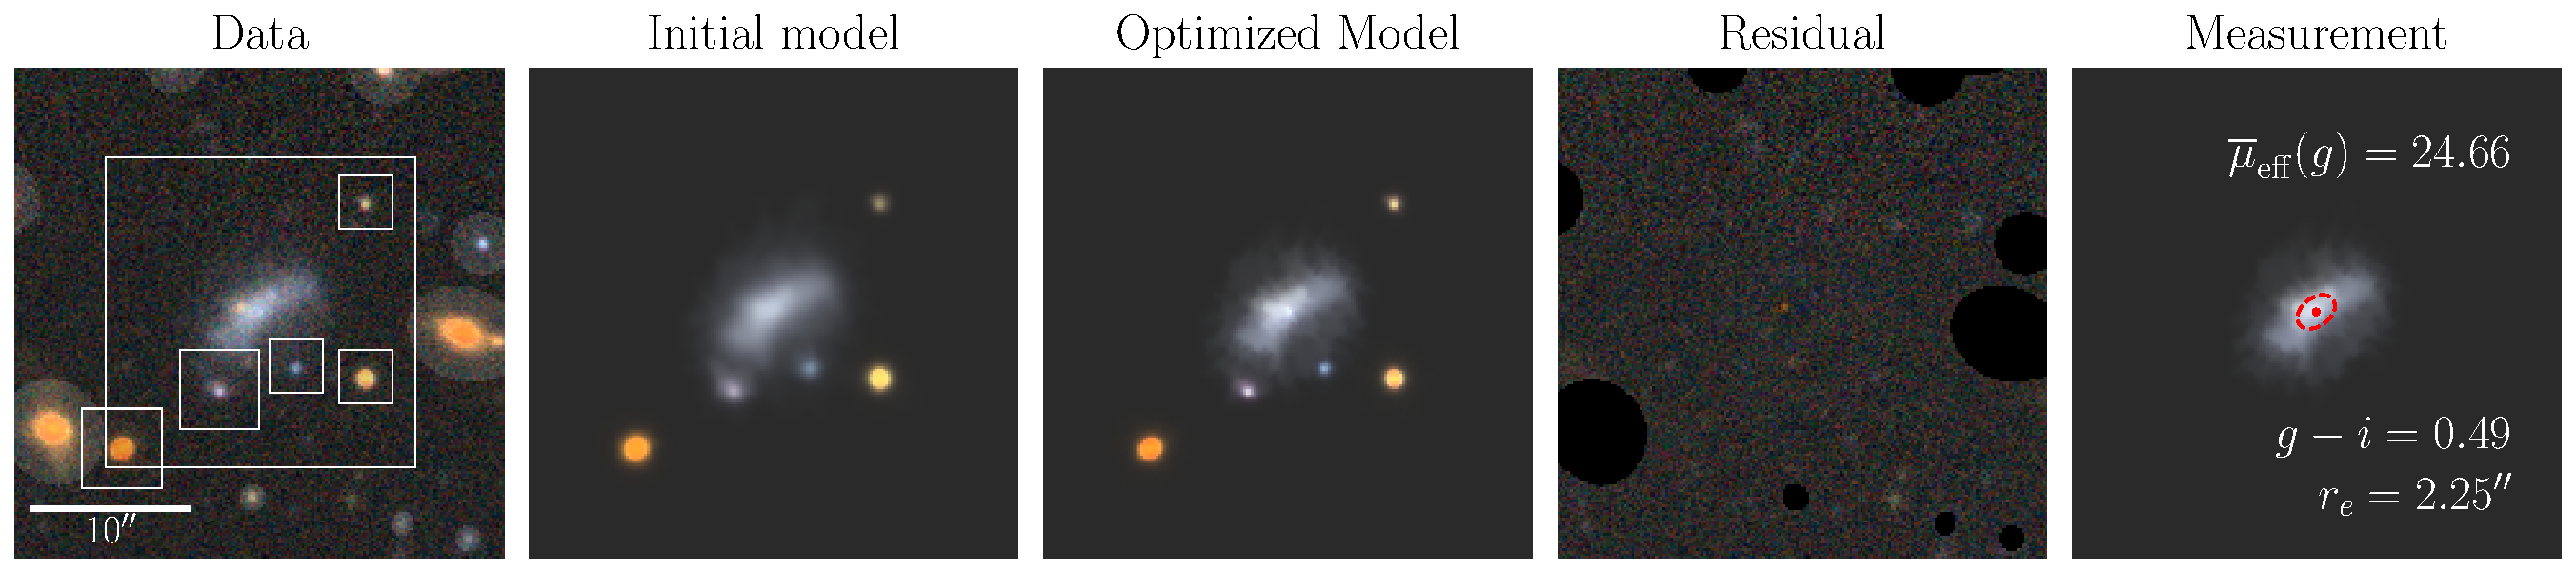
\includegraphics[width=1\linewidth]{vanilla_scarlet_demo.pdf}
		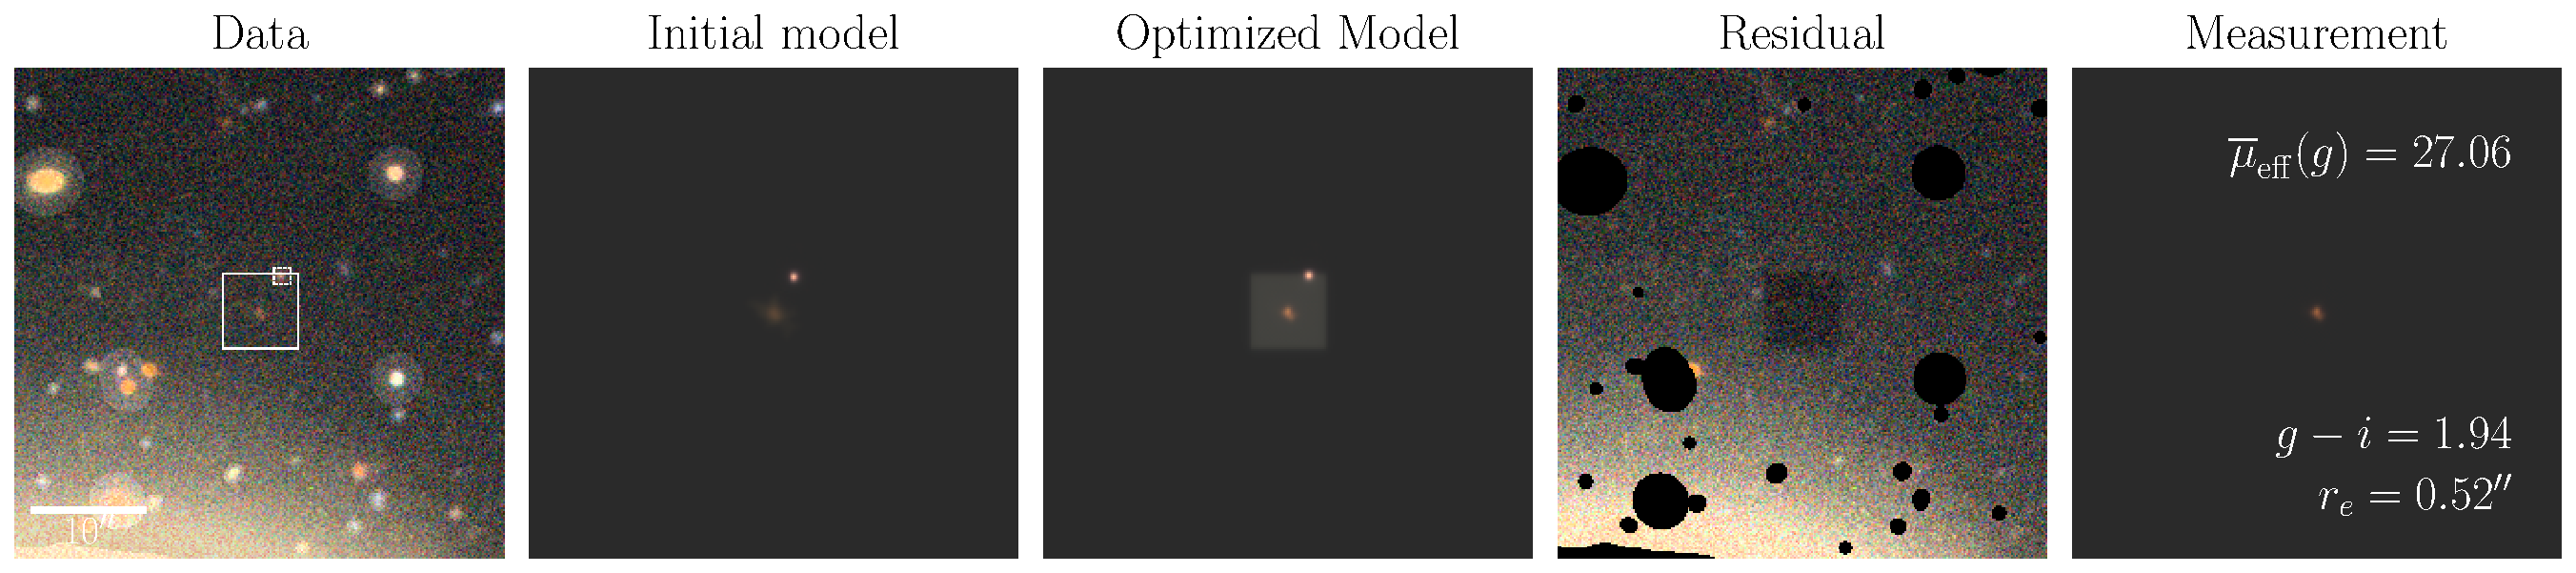
\includegraphics[width=1\linewidth]{vanilla_scarlet_demo2.pdf}
	}
	\caption{An example of the deblending step.}
	\label{fig:vanilla_scarlet_demo}
\end{figure*}


\subsubsection{Measurement and false positive removal}\label{sec:non-par-measurement}
After running vanilla scarlet, we get non-parametric models of objects within the bounding box of the target. We take out the model of the target galaxy (as shown in Figure \ref{fig:vanilla_scarlet_demo}) and analyze it using \code{statmorph}\footnote{\url{https://statmorph.readthedocs.io/en/latest/}}\citep{statmorph}. The goal of this step is to remove false positives using various morphological and structural diagnostics.

\code{Statmorph} calculates non-parametric morphological and structural parameters, including the half-light radius, concentration-asymmetry-smoothness (CAS) statistics \citep{Conselice2003}, Gini-M20 \citep{Lotz2004}, etc. It takes an image, a segmentation map indicating the footprint of the object, a variance map, and PSF. For our purpose, the image is just the scarlet model convolved with the observed PSF. This image represents the deblended target galaxy. Because there is no contaminants in the deblended model, the segmentation map just covers the whole image. The variance map and PSF are taken from HSC cutouts. We also force the sky level to be zero because sky has already been fit in vanilla scarlet. 

One of the most important diagnostics is the size of the object. Half-light radius is calculated using ellpitical apertures, where the ellipticity $\varepsilon$ is determined by calculating the second moment of the image. We define the circularized half-light radius $r_e$ as the geometrical average of the semi-major and semi-minor axis of the half-light elliptical aperture: $r_e = r_{\rm sma} \sqrt{b/a}$. The total magnitudes are simply calculated by summing up the model in each band, and colors are defined by the difference among apparent magnitudes. Galactic extinction correction is not applied at this point. Two kinds of surface brightnesses are measured. The central surface brightness $\mu_0$ is measured by extrapolating the surface brightness profile to $r\to 0$. We also define the average surface brightness within effective radius as $\mu_{\rm eff} = m - 2.5 \log_{10}(2 \pi r_e^2)$, where $m$ is the total magnitude. 

We also use Gini-M20 and CAS statistics. The Gini coefficient \citep{Abraham2003,Lotz2004} and M20 statistics quantify how concentrated/extended is the flux distribution across the image. The CAS statistics characterize the concentration ($C = 5\log_{10}(r_{80} / r_{20}$), asymmetry, and smoothness of the light distribution of the object. We refer the readers to \citet{statmorph} for more details on their definitions and implementations. The morphological and structural parameters are the same in different bands by design of the \code{scarlet} model.


To better guide us on how to use these diagnostics, we visually inspected a subset of LSBG candiates in our initial sample (Sec \ref{sec:detection}) and use the labels to construct the metrics. We randomly selected 5,000 LSBG candidates that are matched with a host at $0.02 < z < 0.04$ (see Sec \ref{sec:match} for details). We run vanilla scarlet and measure morphological parameters for this subsample as described above. Then we generate color composite image for each object using HSC $griz$-bands with 0.5 arcmin on a side. The visual inspection was done by coauthors JEG, JG, SH, RB. Each object has been inspected by at least one person. Objects are classified into three types: \code{candy} (LSB galaxies with typicall dwarf galaxy features), \code{galaxy} (high surface brightness galaxies, or galaxies with spiral galaxy features), \code{junk} (false positives, including tidal streams, galaxy outskirts, and other artifacts). The difference between \code{candy} and \code{galaxy} can be quite ambiguous. In the end, we combine the votes from different persons as follows. An object is classified as \code{junk} if the number of votes as \code{junk} prevails the number of votes as \code{candy} and \code{galaxy}. For objects that are not \code{junk}, if the number of votes as \code{candy} is larger than that as \code{galaxy}, we assign this object as \code{candy}. Everything else is classified as \code{galaxy}. In total, there are 1146 \code{candies}, 2146 \code{galaxies}, and 1708 \code{junks}.

We use this visual inspection results to guide us on using the morphological and structural diagnostics. The distributions of \code{candy}, \code{galaxy}, and \code{junk} in the parameter space are shown in the top panels of Figure \ref{fig:deblending_cuts}. False positives (\code{junk}) are highlighted in red. Altough false positives are scattered all over the parameter space, a large fraction of them occupy regions with small size, extreme colors, very faint surface brightness, and large concentration and asymmetry. Therefore, we come up the following selection cuts to remove the false positives:
\begin{itemize}
    \item Color:
    \[0.0 < g-i < 1.2,\quad |(g-r) - 0.7\cdot (g-i)| < 0.25\]
    \item Size: \[1.8 \arcsec < r_e < 12 \arcsec\]
    \item Surface brightness: \[\mu_0(g) > 22.5,\quad 23.0 < \mu_{\rm eff}(g) < 27.5,\]
    \item Morphology: 
    \begin{gather*}
        \varepsilon < 0.65,\quad \mathrm{Gini} < 0.70,\quad M_{20} < -1.1,\\
        \mathrm{Gini} < -0.136\cdot M_{20} + 0.37,\\
        1.8 < C < 3.5,\quad A < 0.8.
    \end{gather*}
\end{itemize}
These criteria (shown as dashed lines) effectively help us remove objects that are not likely being LSBGs of interest. The color cuts here is narrower than the one used in detection to further remove junks and background high redshift galaxies. It is worth noticing that we not only remove objects with small sizes, but also remove objects with large size, low surface brightness, and high concentration. This is because the scarlet model of some junks can be very concentrated in the center but also extends quite far. The slant demarcation line on Gini-$M_{20}$ diagram is motivated by the line used in \citet{Lotz2008} to seperate merging galaxies and normal galaxies. 

The distributions of objects after applying the above cuts are shown in the bottom panels of Figure \ref{fig:deblending_cuts}. After the cuts, 97\% of the \code{junk} are removed, but the majority (70\%) of \code{candy} still remains. The number of \code{galaxy} also drops by 75\%. This empirical selection based on the non-parametric measurements on the scarlet models successfully removes most of the false positives and a large fraction of background galaxies in our initial sample. The numbers used in the selection are purely driven by the visual inspection results. 

It is worthy noticing that the scarlet modeling and non-parametric measurements is not designed to recover the intrinsic properties of the galaxies. They are only used as a diagnotic tool to remove false positives. Therefore, the half-light radius measured above does not correspond to the half-light radius of the galaxy itself, but merely a proxy. In reality, the vanilla scarlet model usually under-estimates the size and the total flux of LSB objects because the faint outskirts are typically not modeled well due to the non-parametric nature of vanilla scarlet and the monotonicity constraint. In Section \ref{sec:modeling}, we propose a method to better measure the size and total magnitude of LSBG using \code{scarlet}. We use the parameters measured in Section \ref{sec:modeling} for science. 

\begin{figure*}
	\vbox{ 
		%\vskip -10mm
		\centering
		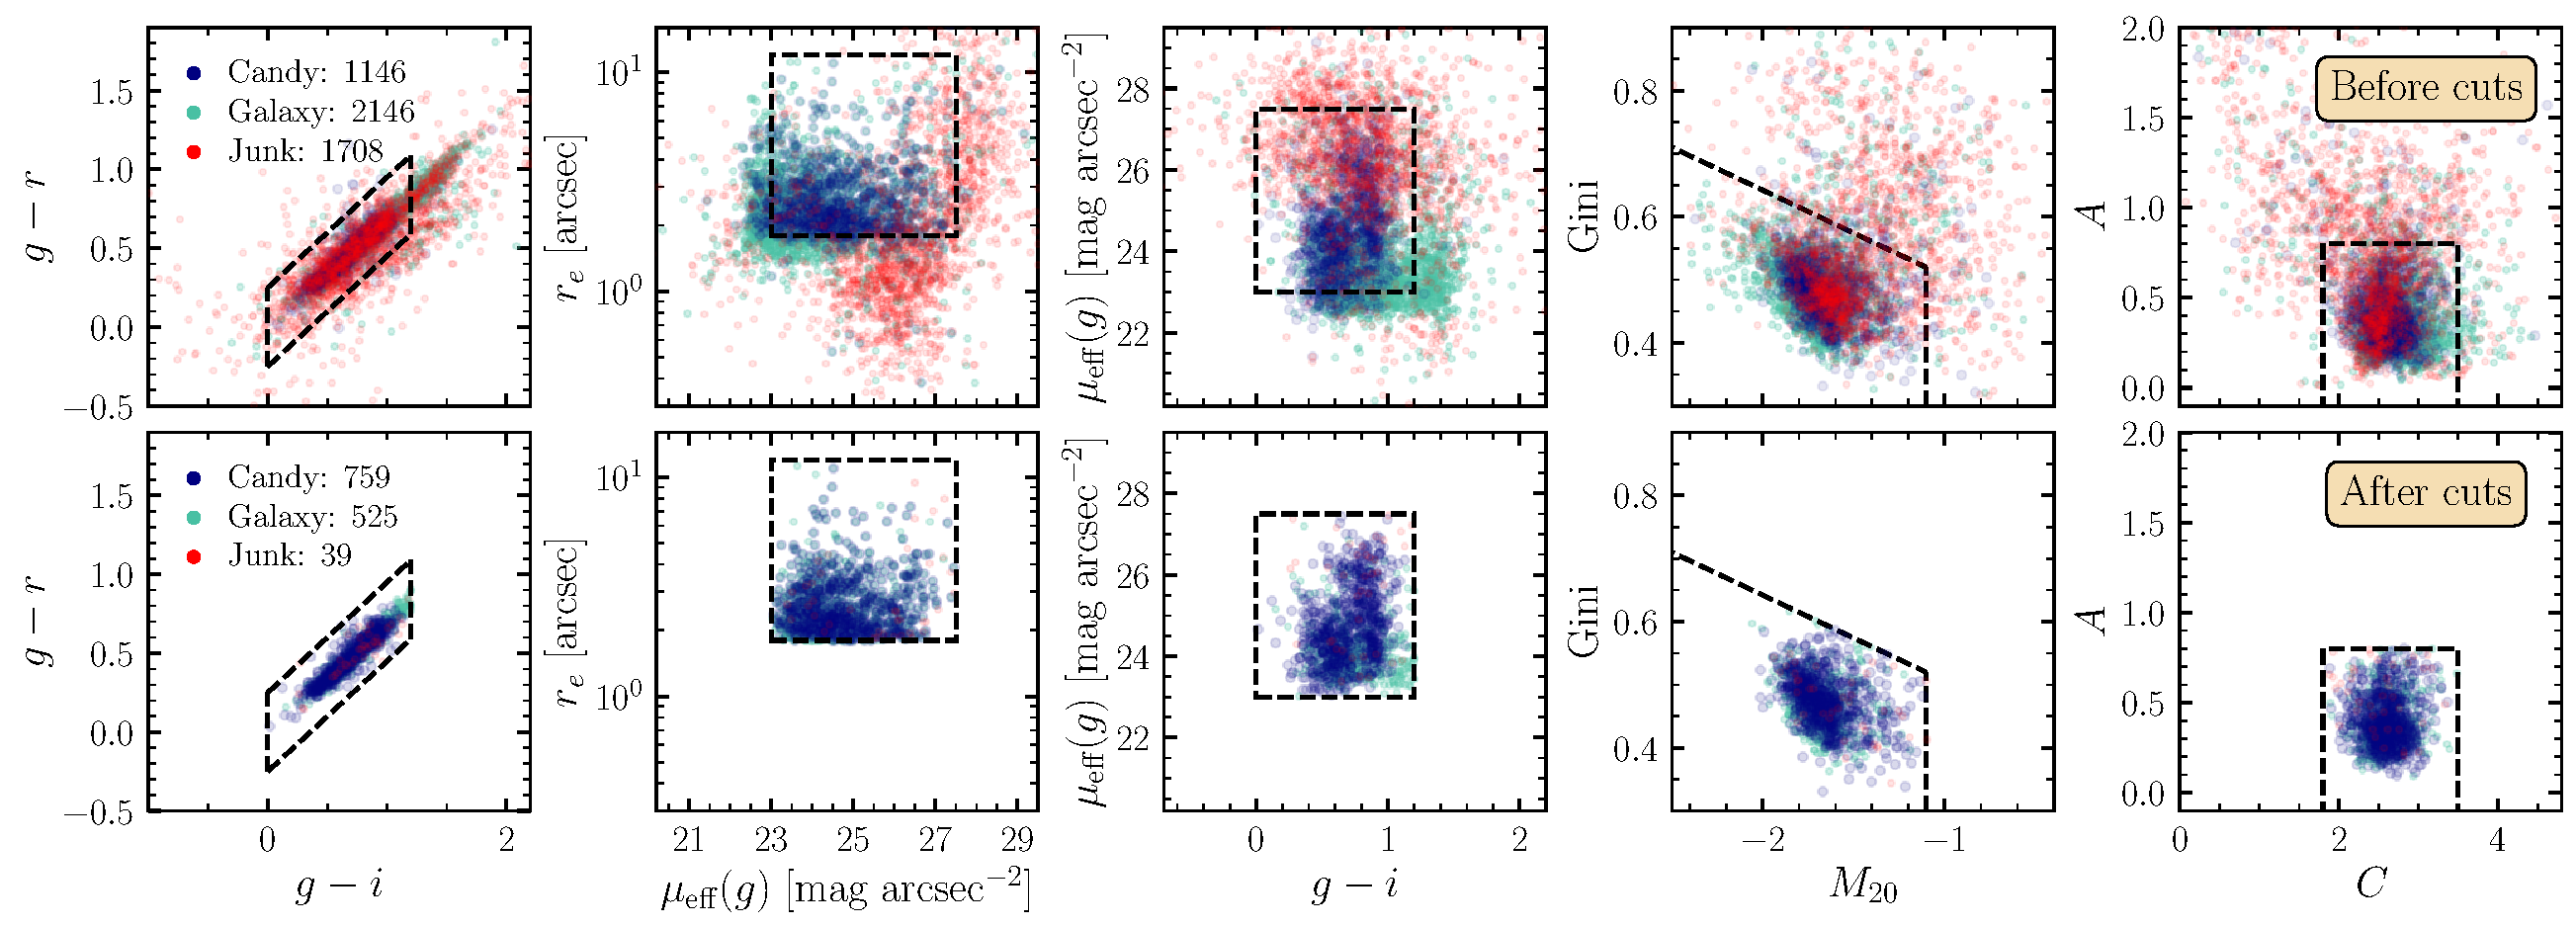
\includegraphics[width=1.0\linewidth]{deblending_cuts.pdf}
	}
	\caption{Deblending cuts.}
	\label{fig:deblending_cuts}
\end{figure*}


Common false positives: why we want a deblending step

Why use scarlet: color info, non-par, monotonic, standard in future HSC, fast, high success rate. Vanilla scarlet.

We do not do scarlet fitting for the entire initial sample, because time consuming. We first match with MW hosts. 


\subsection{Modeling}\label{sec:modeling}
Although vanilla scarlet does a good job on removing false positives, the measured size, magnitude, and surface brightness on the vanilla scarlet model are quite biased. These measurements cannot be used to derive the physical properties of LSBGs. 

The non-parametric modeling in \code{scarlet} assumes weak correlation between pixels by imposing the monotonicity constraint. This leads to two problems when applying vanilla scarlet to the LSBGs. First, since pixels are not strongly correlated in the model, the model cannot capture the galaxy light at very low signal-to-noise ratio. Second, the monotonicity constraint stops the model to grow in certain directions if there is another source along this direction, otherwise the monotonicity is broken. This issue, dubbed as the ``cookie-cutter effect'', can be seen in Figure \ref{fig:vanilla_scarlet_demo}. As a result, the non-parametric model often does not capture the LSB outskirts of LSBG, thus biases the measuremenets. 

On the other side, parametric modeling imposes a very strong correlation on pixels. For example, using a 1-D light profile such as \sersic{}, pixels within an isophote are assumed to have the same intensity. Therefore, the signal-to-noise ratio in the outskirts is boosted by effectively combing the information from many pixels. The parametric model also does not suffer from the ``cookie-cutter'' issue. 

A traditional way of doing parametric modeling is to first mask out contaminants based on the detection segmentation map, then fit a model to the masked image. However, the fitting results are very sensitive to the masking scheme \citep[e.g.,][]{Greco2018}. A possible solution to this problem is to model all the objects in the cutout simultaneously using parametric models (e.g., in DECaLS, \citealt{Dey2019}). In this work, we combine the advantage of parametric modeling with the power of deblending in \code{scarlet}. To be specific, we follow the spirit of deblending as described in Section \ref{sec:deblending}, but replace the non-parametric model for the target with a parametric model. In this way, the LSB outskirts of LSBGs can be better captured with the parametric model and the impact of contaminants is minimized. 

We use the Spergel light profile to model the LSBGs. The Spergel profile is motivated by having a simple analytical expression in Fourier space, making it easy to be convolved with a PSF.\footnote{On the opposite, the \sersic{} profile does not have a simple analytic form in Fourier space.} The surface brightness of a Spergel profile \citep{Spergel2010} has a form of
\begin{equation}
    \label{eq:spergel}
    I_\nu(r) = \frac{c_{\nu}^{2} L_{0}}{2\pi r_{0}^{2}} f_{\nu}\left(\frac{c_{\nu} r}{r_{0}}\right),
\end{equation}
where 
\begin{equation}
    f_{\nu}(u)=\left(\frac{u}{2}\right)^{\nu} \frac{K_{\nu}(u)}{\Gamma(\nu+1)},
\end{equation}
and $K_\nu(u)$ is the Modified Bessel function of the second kind. The half-light radius is $r_0$, the total luminosity is $L_0$, and $c_\nu$ satisfyies the equation $(1 + \nu)f_{\nu + 1}(c_\nu) = 1/4$. Similar to the \sersic{} index, the parameter $\nu$ (Spergel index) controls the concentration of the light profile. As shown in Appendix \ref{ap:spergel}, the Spergel profile approximates the \sersic{} profile very well over the range of \sersic{} index that is interested to the study of LSBGs.

There are several changes in the modeling compared to the deblending step. First, we intialize a vanilla scarlet model for the target object as in Section \ref{sec:deblending}. Then we measure the half-light radius, total flux, and shape of the scarlet model. We use these numbers to initialize the Spergel profile. The size of the bounding box is also updated to be the maximum between 250 pixel and $10\, r_e$. Objects within this bounding box are included in the modeling, but only the target object is modeled by the Spergel profile. For the target, we still requires positivity constraint, as the mononicity is automatically satisfied. 

After optimization, we take the $r_0$ in Equation \eqref{eq:spergel} as the circularized half-light radius $r_e$, and take the $L_0$ as the total flux. The average surface brightness $\overline{\mu}_{\rm eff}$ is calculated in the same way as in Section \ref{sec:non-par-measurement}. 

We characterize the quality of the Spergel modeling by injecting mock \sersic{} galaxies into the cutout and compare the recovered properties with the truth, as shown in Appendix \ref{sec:meas_unc}. Overall speaking, the measurement agrees with the truth quite well. However, the size and the total flux of galaxies below $\overline{\mu}_{\rm eff} (g) > 27$ is under-estiamted. We also characterize the bias and the scatter in measurement as a function of size and surface brightness. We apply the bias correction to the measurement of LSBGs, and incorporate the measurement error into the science figures. 

\subsection{Completeness and Measurement Uncertainty}

\subsubsection{Completeness}\label{sec:completeness}
\begin{figure*}
	\vbox{ 
		%\vskip -10mm
		\centering
		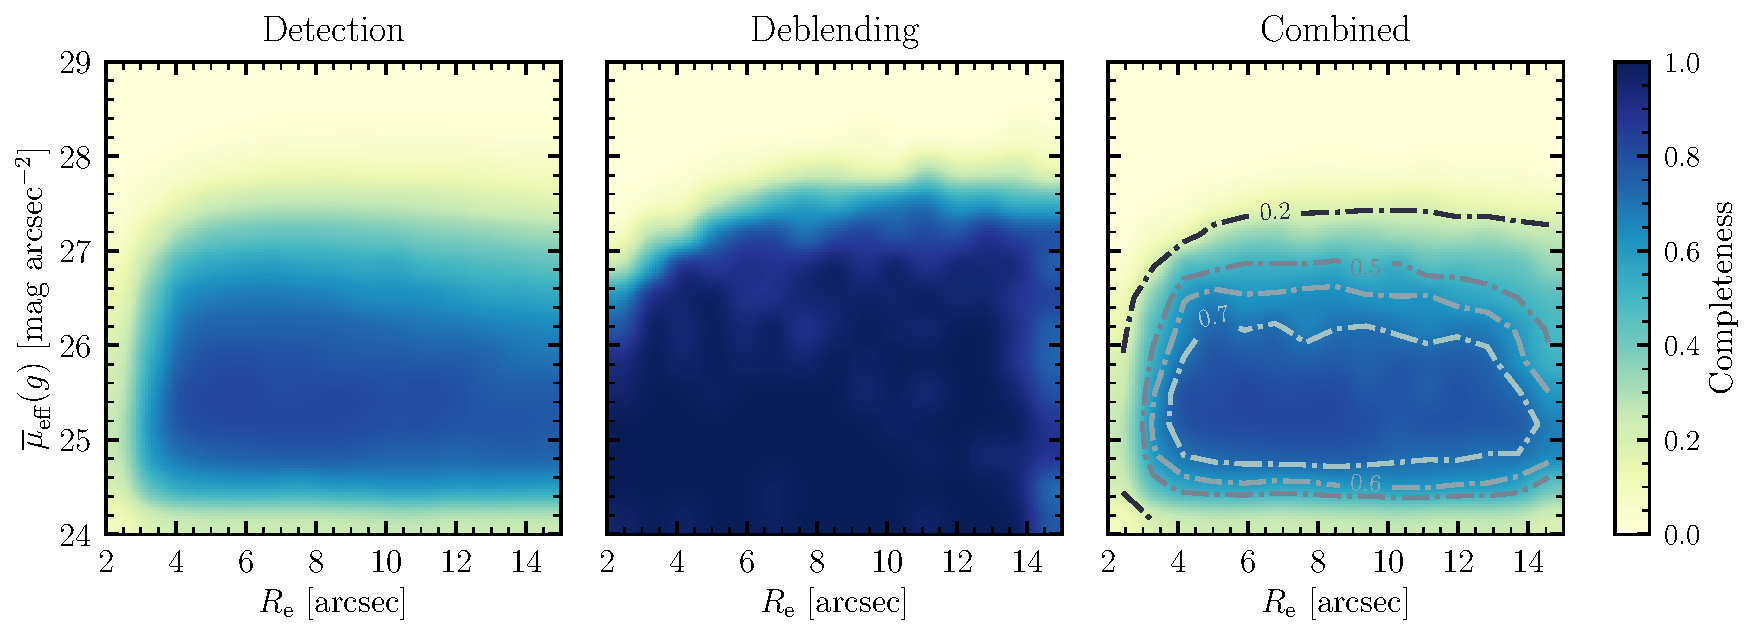
\includegraphics[width=1\linewidth]{completeness.pdf}
	}
	\caption{Caption}
	\label{fig:completeness}
\end{figure*}

%Since the scarlet model is PSF-deconvolved, the color is not affected by the seeing differences among bands. 
After the source detection step and the deblending step, we obtain a sample of LSBG candidates where the fraction of false positives is very small. 

It is crucial to characterize the completeness of both detection and deblending in order to understand our survey efficiency and the properties of the LSBG population. We performed a large suite of image simulation to derive the completeness. The overall completeness is a combination of detection and deblending completenesses. The detection completeness is defined as the number of detected objects divided by the number of injected objects, whereas the deblending completeness is defined as the fraction of objects remained after cuts. 

For the detection completeness, we inject $\sim 35,000$ (check number with Johnny) mock galaxies with single \sersic{} light profiles \citep{Sersic1963} into the coadd images\footnote{We have also done extensive tests on injecting mock galaxies to the raw images and going through the entire data reduction pipeline. This is very expensive in terms of both CPU time and disk space, since we must run the full \code{hscPipe}. However, we find no noticable difference between this method and the direct injection to coadd images.}. The mock galaxies follow uniform distributions in size ($2\arcsec \leqslant r_{e} \leqslant 21\arcsec$), surface brightness ($23 \leqslant \overline{\mu}_{\rm eff}(g) \leqslant 28.5\ \mathrm{mag\ arcsec^{-2}}$), \sersic{} index ($0.8 < n < 1.2$), and ellipticity ($0 < \epsilon < 0.6$), resembling the LSBG distribution in \citetalias{Greco2018}. They are randomly assigned to have a blue ($g-i=0.47,\ g-r=0.32$) and red ($g-i=0.82,\ g-r=0.56$) color with equal chance.

We find the detection completeness mainly depends the size and surface brightness of mock galaxy. As shown in the left panel of Figure \ref{fig:completeness}, the detection completeness remains high across different sizes. It drops below 50\% when the surface brightness gets fainter than 27.5 mag arcsec$^{-2}$. We find negligible dependendce of completeness on \sersic{} index, color, and additional structure of galaxy (such as star-forming clumps). However, we find the completeness declines above ellipticity $\varepsilon > 0.6$, suggesting that edge-on disk galaxies may be missing from our sample. In this work, we neglect the dependences of detection completeness on parameters other than size and surface brightness. 

\textbf{Need to update the completeness to the S18A version. Ping Johnny.}

For the deblending completeness, we inject 5,000 mock \sersic{} galaxies into the coadd and run vanilla scarlet on them. The mock galaxies follow the same uniform distribution in size, surface brightness, ellipticity, \sersic{} index as for deriving the detection completeness, but follow a Gaussian distribution in color: $g-i \sim \mathcal{N}(0.6, 0.2^2),\ g-r = 0.7 (g-i) + \mathcal{N}(0, 0.03^2)$. Following the procedure described in Sec \ref{sec:deblending}, we measure the non-parametric sizes and surface brightnesses on the scarlet models of the mock galaxies. The deblending completeness is shown in the middel panel of Figure \ref{fig:completeness}. The deblending completeness is high at bright surface brightnesses, but starts to decline with increasing size and surface brightness. Mock galaxies fainter than $\overline{\mu}_{\rm eff}(g) > 27.5$ are mostly removed by the deblending step, likely due to the blending of other small compact sources with the mock galaxy. The deblending step is very effective on removing false positives, but at a cost of losing very LSB galaxies. 

The combined completeness is shown in the right panel of Figure \ref{fig:completeness}. The countours shows the 70\%, 50\%, and 20\% completenesses, respectively. \textbf{Also compare our completeness with other surveys.}

%\textbf{Make sure that completeness is assigned based on the bias-corrected size and SB.} Checked. No problem.

\subsubsection{Measurement uncertainty}\label{sec:meas_unc}
We characterize the quality of the Spergel modeling by injecting mock \sersic{} galaxies into the cutout and compare the recovered properties with the truth, as shown in Appendix \ref{sec:meas_unc}. Overall speaking, the measurement agrees with the truth quite well. However, the size and the total flux of galaxies below $\overline{\mu}_{\rm eff} (g) > 27$\sbunit is under-estiamted. We also characterize the bias and the scatter in measurement as a function of size and surface brightness. We apply the bias correction to the measurement of LSBGs, and incorporate the measurement error into the science figures. 

In order to test how well do we recover the photometric and structural parameters in the modeling step (Sec \ref{sec:modeling}), we take the 5,000 mock \sersic{} galaxies used for computing the deblending completeness and model them using the Spergel light profile. We compare the fitting results with the ground truth in Figure \ref{fig:meas_bias}, where $\Delta(X) = X(\rm truth) - X(\rm measured)$, and x-axis corresponds to the truth values. We find that the measured half-light radius $r_e$ is biased to be smaller than the truth, and the bias depends on the surface brightness and apparent size. For surface brightness fainter than 27\ \sbunit, the measured size can be much smaller than the truth. As a result, the apparent magnitude $m$ and the average surface brightness $\overline{\mu}_{\rm eff}$ are also measured to be fainter than the truth. 

To correct for this bias in size, surface brightness, apparant magnitude, and color, we assume that the bias only depends on the size and surface brightness. Indeed, we do not find any significant dependence of the bias on color, ellpticity, and Spergel index. We split the $r_e-\overline{\mu}_{\rm eff}(g)$ plane using a $8\times 8$ grid, and calculate the mean bias within each bin. Then we interpolate over the grid using a multiquadratic kernel\footnote{\url{https://docs.scipy.org/doc/scipy/reference/generated/scipy.interpolate.RBFInterpolator.html}}. Figure \ref{fig:meas_err} shows the interpolated bias terms as a function of the measured size and surface brightness. For half-light radius, we take $(r_{e, \rm t} - r_{e, \rm m}) / r_{e,\rm m}$ as the bias term; for surface brightness, we take $\overline{\mu}_{\rm eff, t}(g) - \overline{\mu}_{\rm eff, m}(g)$ as the bias term. As shown in Figure \ref{fig:meas_err}, the size and surface brightness bias grows as increasing surface brightness. The bias has a peak at $r_e\sim 6\arcsec$ because the $r_e$ shown in the figure is the measured size, not the truth size. It is the bias in size measurement that makes galaxies with large intrinsic $r_e$ pile up around $r_e\sim 6\arcsec$. We also find that the bias in $g-i$ color is quite small. 

For LSBGs in our sample, we apply corrections for the bias using the interpolated bias terms. We first correct for the bias in size, $g$-band average surface brightness, $g-r$ and $g-i$ colors. Then we calculate the $g$-band apparent magnitude following $m_g = \overline{\mu}_{\rm eff}(g) - 2.5\log(2\pi r_e^2)$. The magnitudes and surface brightnesses in other bands are derived using $g$-band magnitude, surface brightness, and colors. In this way, we apply a self-consistent correction for the measurement bias to the data. 

Besides, it is also important to characterize the measurement uncertainty. The measurement uncertainty consists of a statistical uncertainty which is determined by the shape of the likelihood (posterior) surface, and a systematic uncertainty which is related to various factors including sky subtraction, contamination effects, etc. Unlike other parametric modeling code such as \code{galfit} or \code{imfit}, \code{scarlet} does not explore the full likelihood (posterior) space but rather finds one optimial solution. Thus we cannot get a statistical error of the measured properties from \code{scarlet}. However, by comparing the recovered properties of mock galaxies with the truth, we can empirically estimate the measurement uncertainty without knowing the impact of each factor. Following the same way of calculating the bias, in each bin, we compute the standard deviation of the difference between the truth and the bias-corrected measurement, then we interpolate over the grid. The measurement errors are shown in Figure \ref{fig:meas_err} as contours. 



TBD: re-think the way of computing the error, especially for $r_e$. 


vdB 16 doesn't consider whether GALFIT gives the corrrect $R_e$, when deriving the completeness (recovered fraction)

Remember to ref SMUDGES papers here.

\begin{figure*}
	\vbox{ 
		\centering
		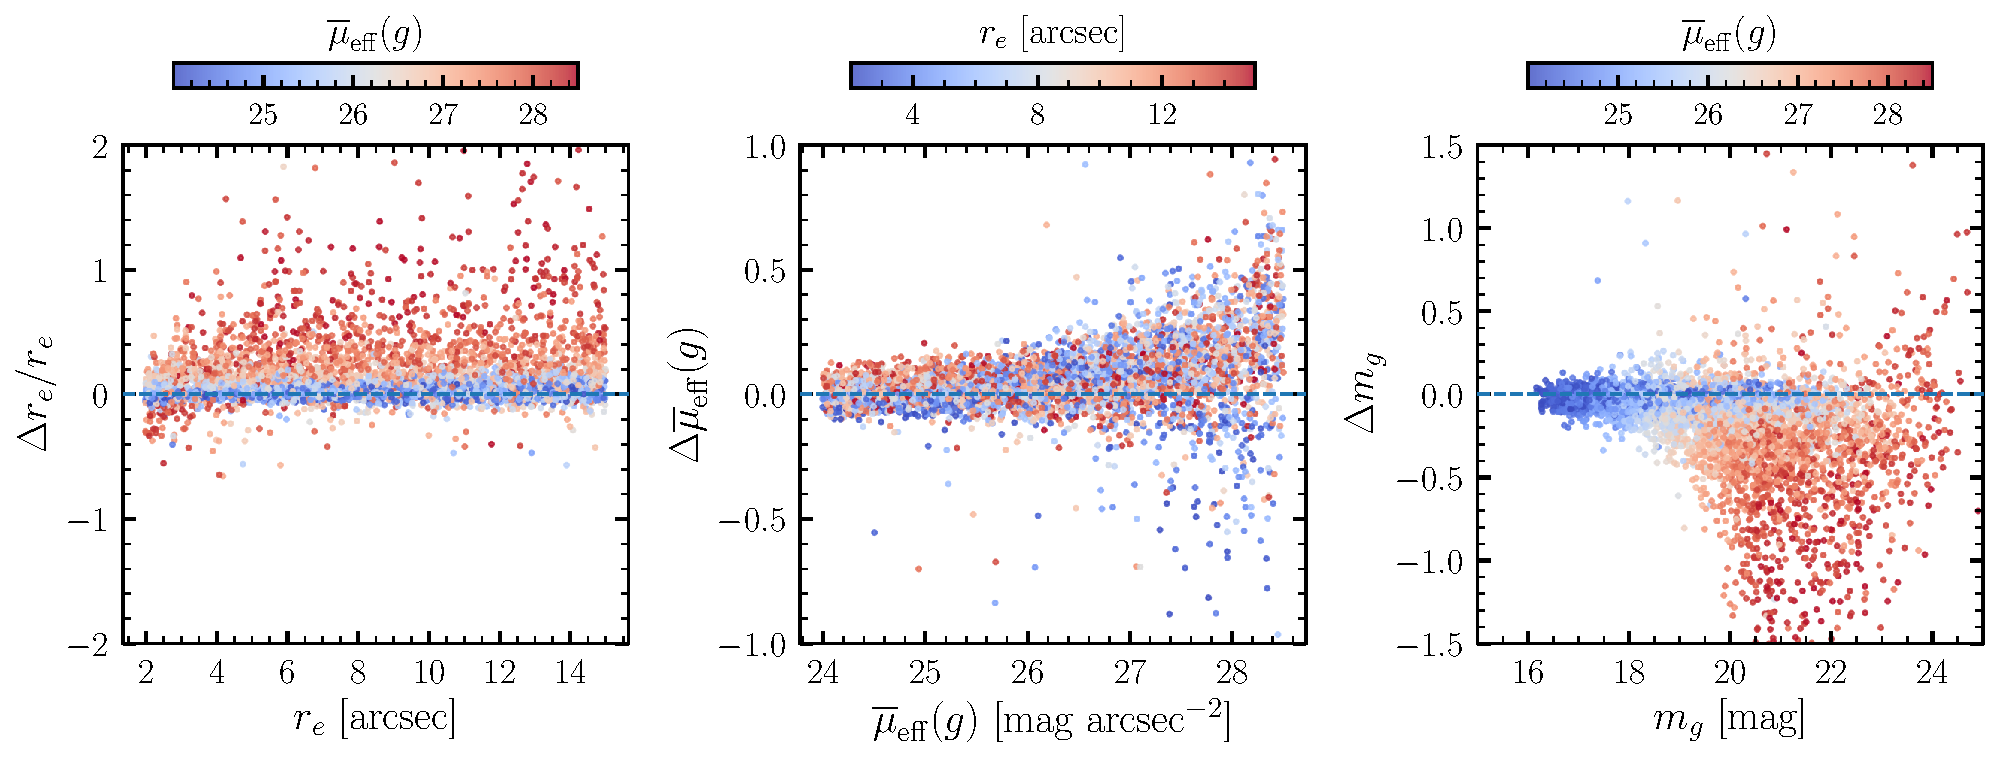
\includegraphics[width=1\linewidth]{meas_bias.pdf}
	}
    \caption{Caption}
    \label{fig:meas_bias}
\end{figure*}


\begin{figure*}
	\vbox{ 
		\centering
		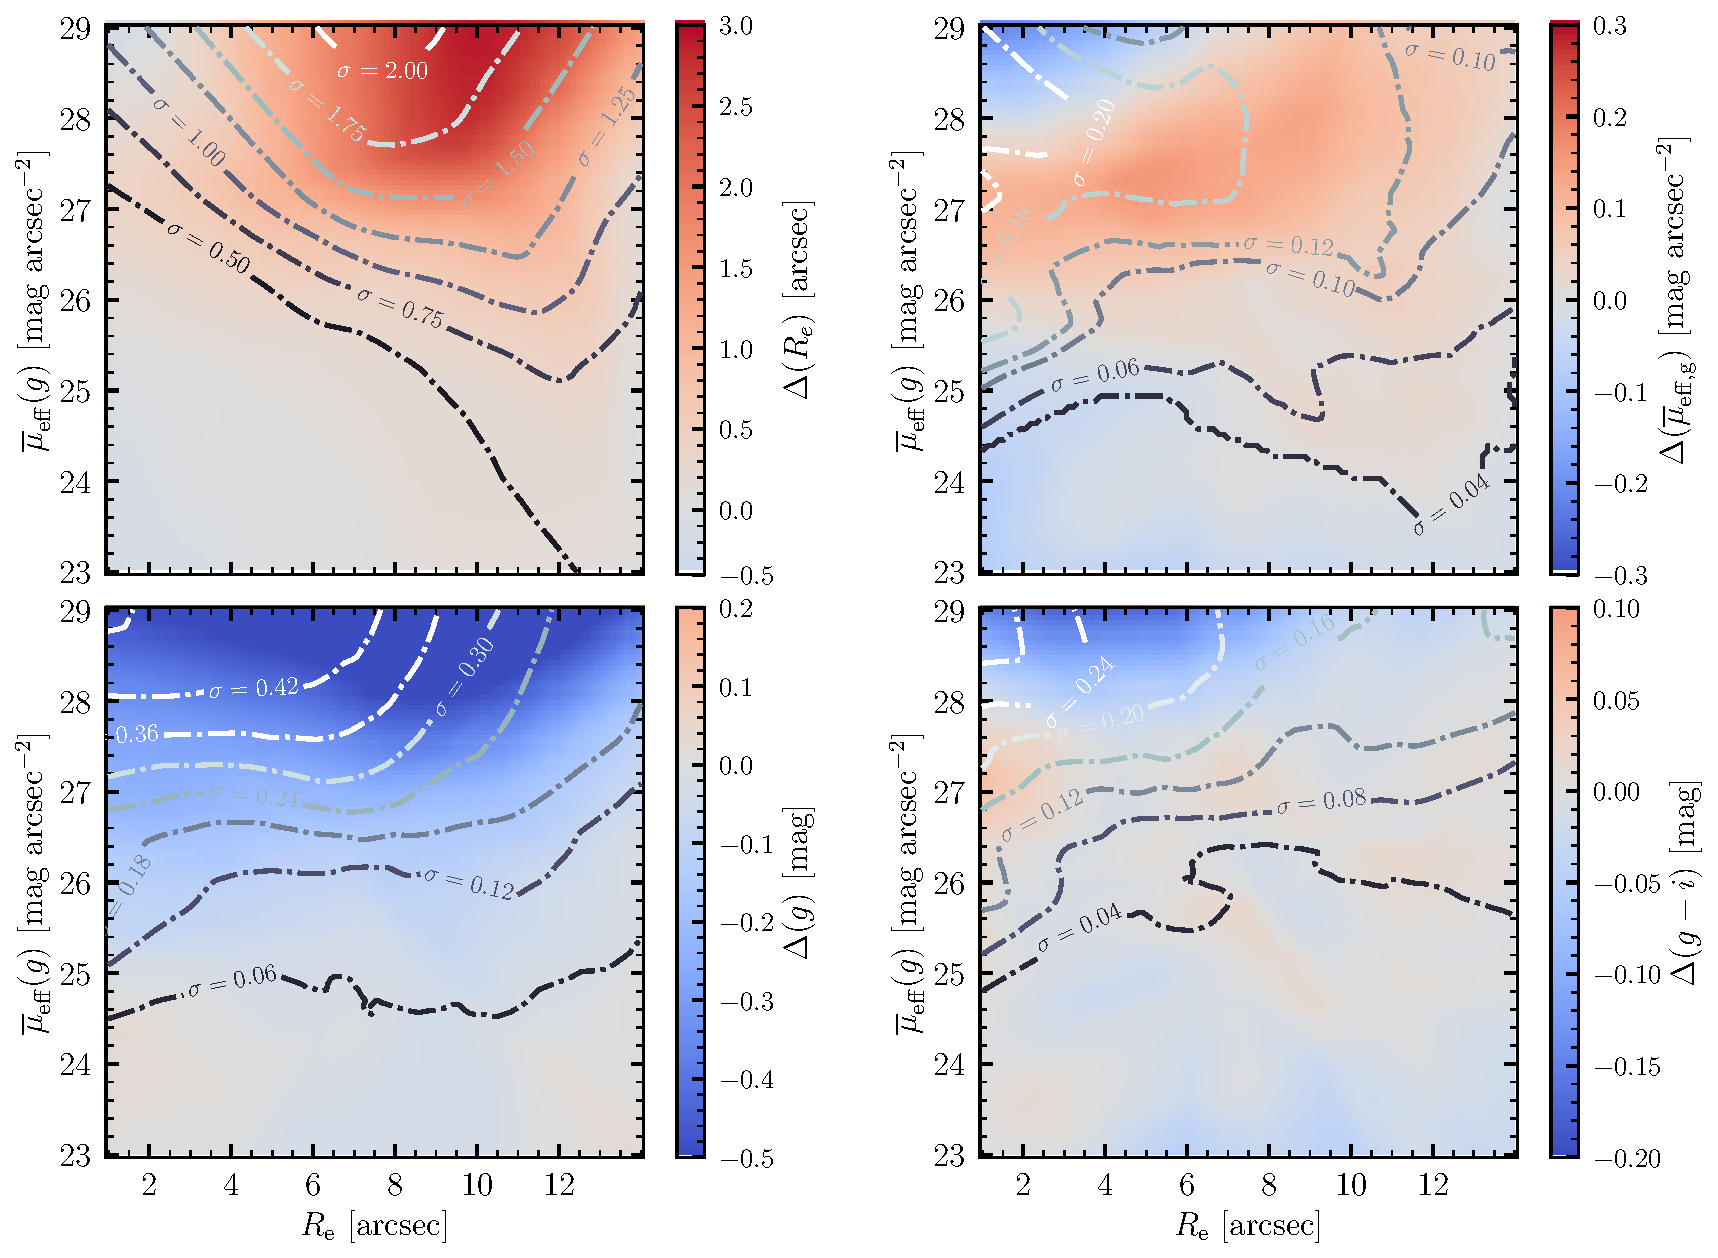
\includegraphics[width=1\linewidth]{meas_error_spergel.pdf}
	}
    \caption{Caption}
    \label{fig:meas_err}
\end{figure*}

\section{UDGs in Milky-Way analogs}

\subsection{Matching with Milky-Way analogs}\label{sec:match}
The goal of this paper is to study the UDG population hosted by MW-like galaxies. However, the properties of MW itself vary in literature \citep{Licquia2015,Bland-Hawthorn2016}, and the definitions of MW analogs are also different among groups. In the SAGA survey \citep{SAGA-I,SAGA-II}, MW analogs are selected based on their absolute $K$-band magnitude $-23 > M_K > -24.6$, which is derived using abundance matching by assuming a simple galaxy-halo connection model (Fig 2 of \citealt{SAGA-I}). This luminosity range approximately corresponds to a stellar mass range of $10.2 < \log\, M_\star/M_\odot < 11.0$. They also require the MW analogs to be in isolation (without nearby bright galaxies) and lie in a redshift range of $0.005 < z < 0.01$ (20-40 Mpc). In the ELVES survey \citep{ELVES-I,ELVES-II,CarlstenELVES2022}, the requirements for MW-like host is loosened to be $M_K < -22.1$ ($M_\star > 10^{9.9}\ M_\odot$) because the probed volume by ELVES ($D<12$ Mpc) is smaller than that of SAGA. We choose the stellar mass range of MW analogs to be $10.2 < \log\, M_\star/M_\odot < 11.2$, which is simply a 1 dex bin centered at the measured stellar mass of the Milky Way ($\sim 10^{10.7}\ M_\odot$, \citealt{Licquia2015}). MW analogs selected using this definition is very close to those in SAGA but are slightly more massive than the ELVES hosts.

Since UDGs are relatively scarce in MW-like hosts \citep{SAGA-II,CarlstenELVES2022}, it is helpful to probe a larger volume to obtain good statistics. However, UDGs will be too small and faint to be detected in HSC images beyond certain distances. We choose our redshift range to be $0.01 < z < 0.04$, which makes sure that we can detect a significant number of faint dwarf galaxies around MW-like hosts. We exclude galaxies $z<0.01$ because 1) the number is very small; 2) their large angular size makes them shredded in deblending step, including them will introduce a lot of spurious LSB objects. Our MW analogs sample complements the ELVES sample and SAGA sample in redshift range. 

After applying the stellar mass and redshift cuts to the NSA catalog, there are 23,218 galaxies left. Then we match them to the LSBG catalog (described in Section \ref{sec:detection}) as follows. For a given MW-like host, we first calculate its virial radius $R_{\rm vir}$ assuming the stellar mass-halo mass relation in \citet{Behroozi2010}. It turns out that 40\% of hosts have virial radii larger than 300 kpc. Then we identify any LSBG that falls into the projected angular virial radius of the host. Then these LSBGs are associated with the host. We repeat this process for all hosts. If one LSBG is associated to multiple hosts, we assign it to the nearest host (normalized by the angular size of virial radius). Finally, we have 901 MW-like hosts and 8,367 LSBG candidates associated with them. However, there are still a significant fraction of spurious objects in this LSBG sample, including galactic cirrus, tidal tails/streams, shrreded large galaxies, compact sources in galaxy outskirts, etc. In the following, we perform a deblending step to effectively remove these spurious objects. 

\subsection{UDG sample and UPG sample}
Remember to filter the UDG sample through the FDFC mask, and also remove duplicated objects.

Also append the catalog.

Plot the UDG and UPG population on the re-abs mag plane (Bovy book)


\begin{figure*}
	\vbox{ 
		\centering
		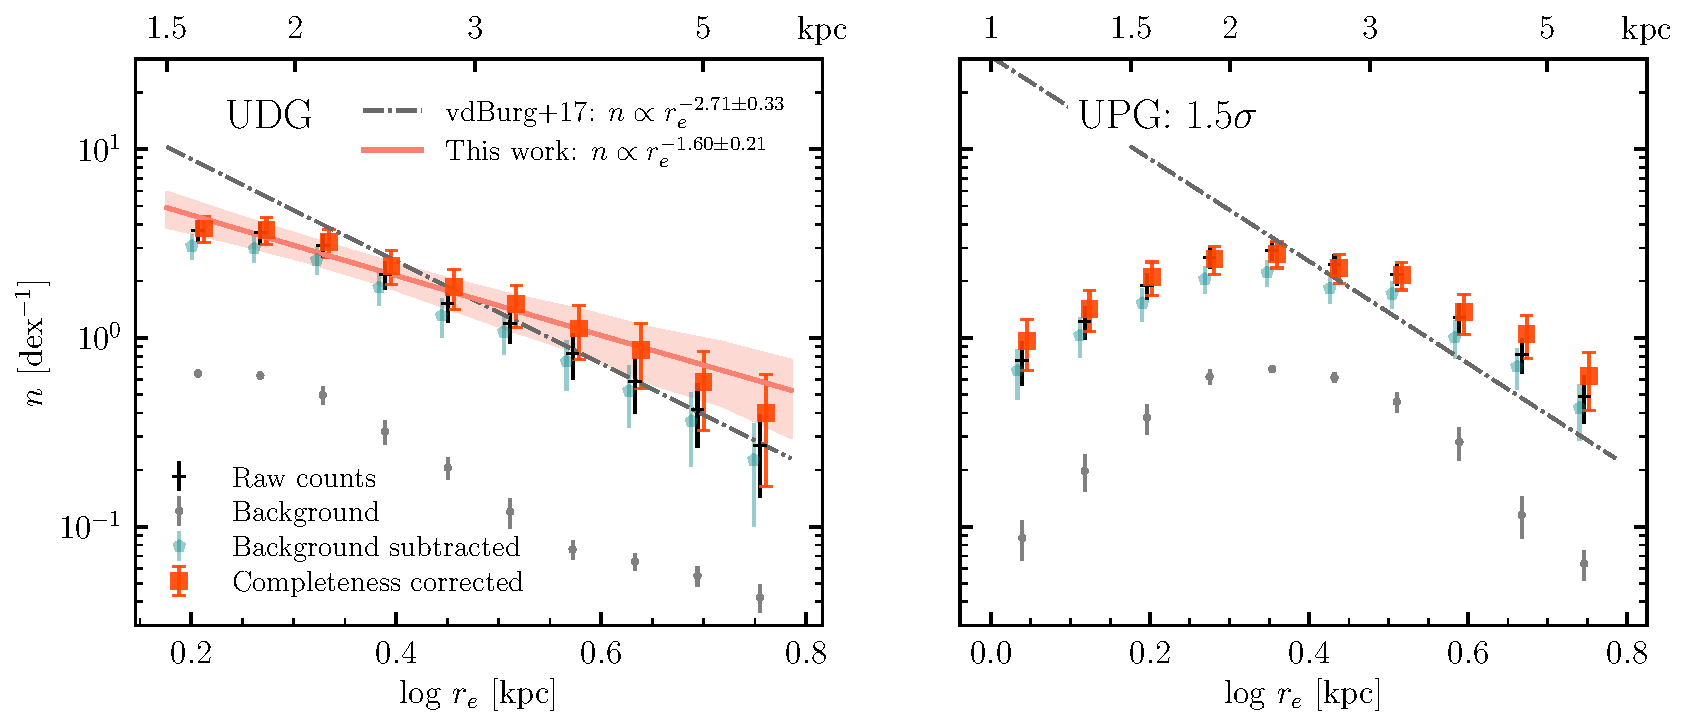
\includegraphics[width=1\linewidth]{size_distribution.pdf}
	}
    \caption{Caption}
    \label{fig:size_distribution}
\end{figure*}


\begin{figure*}
	\vbox{ 
		\centering
		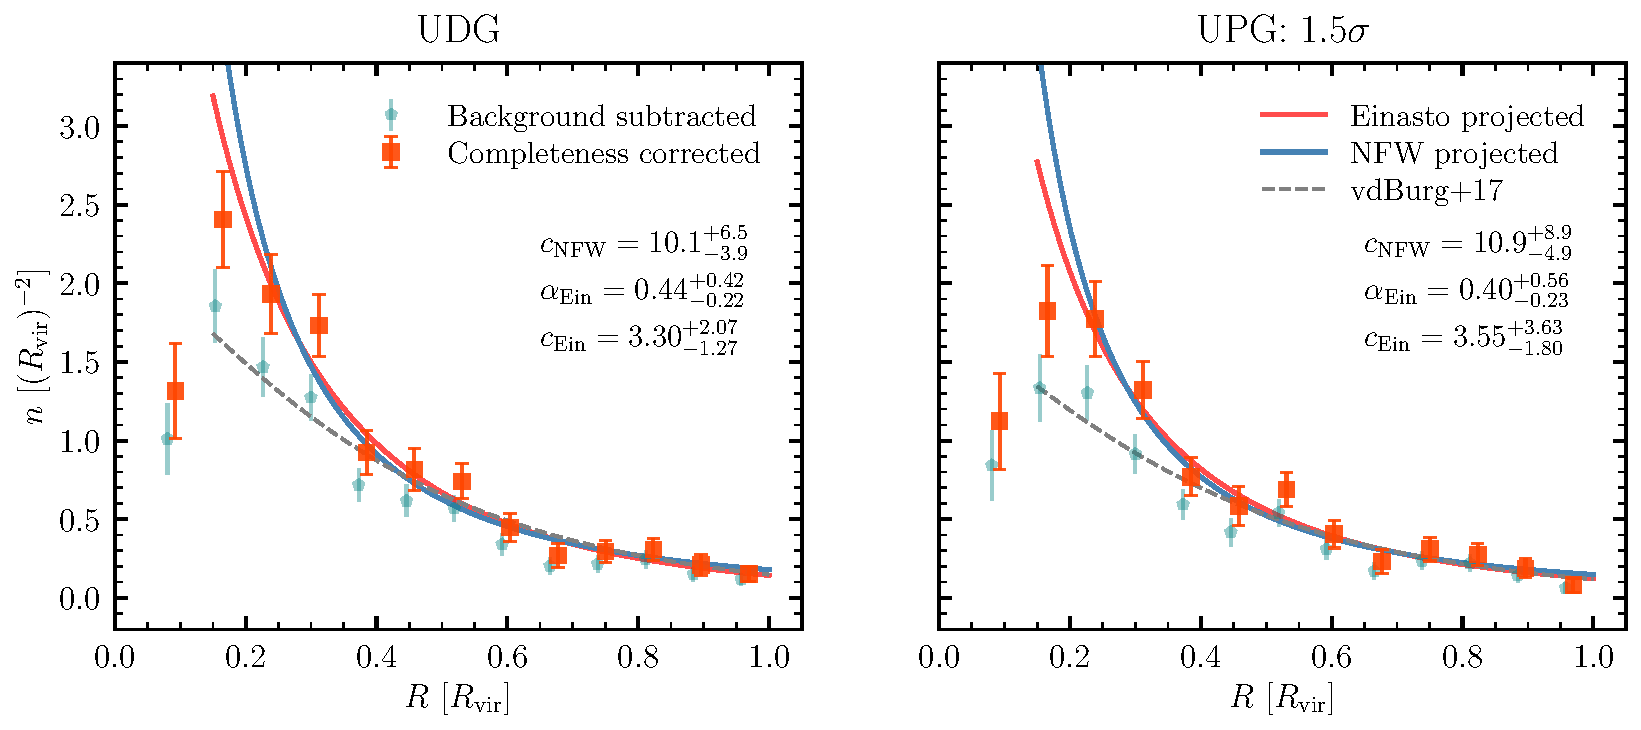
\includegraphics[width=1\linewidth]{radial_distribution.pdf}
	}
    \caption{Caption}
    \label{fig:radial_distribution}
\end{figure*}


\begin{figure*}
	\vbox{ 
		\centering
		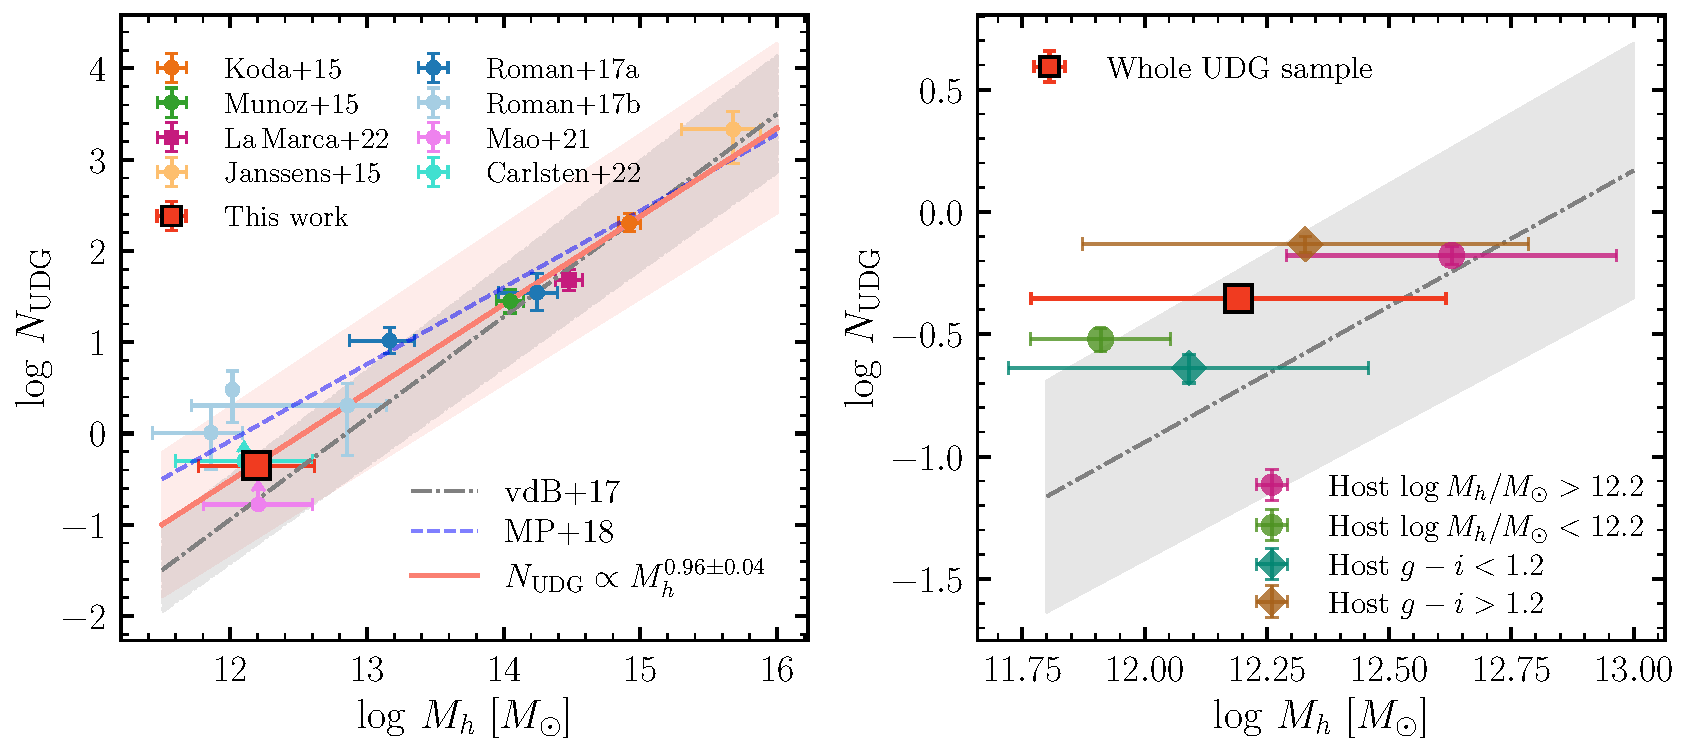
\includegraphics[width=1\linewidth]{N_UDG_host_mass.pdf}
	}
    \caption{Caption}
    \label{fig:n_udg}
\end{figure*}

\subsection{Spatial distribution}

\subsection{Quenched fraction}


\section{Discussion and Conclusion}
Scenarios:
1. violent environmental effects: radial orbits, back-splash both explain large size and quenching. But according to Bernavidis et al, the quenched fraction drops with increasing mass. 

2. accreting field UDGs, and quench them due to ram pressure stripping. But how long do accreted UDGs last before being destroyed? Need to look at ram pressure stripping literature.

Homework:
1. 1.5-sigma definition, UPG
2. number of UDG per host, as a function of host mass bins.
3. Move the stellar mass bin definition, try to match with red/blue, spiral/elliptical plot. If cannot match, does this hint the formation scenarios?
4. How significant do we detect blue UDGs? 
5. Split into redshift bins


TODO:
1. rerun the matching, compensate the left ~1000 LSBGs.
2. galactic extinction. Done!!!

UDG rejuvenate after ram pressure stripping?


Why red is equivalent to quenched? Need to clarify in the paper

calculate probability of being a backsplash satellite (e.g., splashed to 1.5 Mpc)

Compare spatial distribution with normal dwarf? iF they are indeed high-spin tail of normal dwarfs. 




\section*{Acknowledgment}
JL is grateful for discussions with XXX. The authors thank Yao-Yuan Mao for his tool for visualizing image cutouts. 

The Hyper Suprime-Cam (HSC) collaboration includes the astronomical communities of Japan and Taiwan, and Princeton University. The HSC instrumentation and software were developed by National Astronomical Observatory of Japan (NAOJ), Kavli Institute for the Physics and Mathematics of the Universe (Kavli IPMU), University of Tokyo, High Energy Accelerator Research Organization (KEK), Academia Sinica Institute for Astronomy and Astrophysics in Taiwan (ASIAA) and Princeton University.  
Funding was contributed by the FIRST program from Japanese Cabinet Office, Ministry of Education, Culture, Sports, Science and Technology (MEXT), Japan Society for the Promotion of Science (JSPS), Japan Science and Technology Agency (JST), Toray Science Foundation, NAOJ, Kavli IPMU, KEK, ASIAA and Princeton University.
\vspace{1em}
\software{\href{http://www.numpy.org}{\code{NumPy}} \citep{Numpy},
          \href{https://www.astropy.org/}{\code{Astropy}} \citep{astropy}, \href{https://www.scipy.org}{\code{SciPy}} \citep{scipy}, \href{https://matplotlib.org}{\code{Matplotlib}} \citep{matplotlib},
          \href{https://halotools.readthedocs.io/en/latest}{\code{Halotools}} \citep{Hearin2017},
          \href{https://pmelchior.github.io/scarlet/}{\code{scarlet}} \citep{Melchior2018}, \href{https://github.com/dr-guangtou/unagi}{\code{unagi}}.
          }


\bibliography{citation}{}
\bibliographystyle{aasjournal}



\newpage
\appendix 

\section{Spergel profiles}\label{ap:spergel}

In this appendix, we demonstrate that the Spergel profile can approximate \sersic{} profile and profile a lookup table for the correspondence between \sersic{} index $n$ and Spergel index $\nu$.

The surface brightness of a \sersic{} profile follows \citep{Sersic1963,Graham2005}:
\begin{equation}\label{eq:sersic}
    I(r)=I_{\mathrm{e}} \exp \left\{-b_{n}\left[\left(\frac{r}{r_{\mathrm{e}}}\right)^{1 / n}-1\right]\right\},
\end{equation}
where $r_e$ is the half-light radius, $I_e$ is the surface brightness at $r=r_e$, $n$ is the \sersic{} index. The value of $b_n$ satisfies $\Gamma(2 n)=2 \gamma\left(2 n, b_{n}\right)$, where $\gamma(a, x)$ is the incomplete gamma function. According to \citet{Graham2005}, the total luminosity of a \sersic{} profile is given by 
\begin{equation}\label{eq:sersic_lum}
    L_0 = I_{e} r_{e}^{2}\, 2 \pi n\, e^{b_{n}} \left(b_{n}\right)^{-2 n} \Gamma(2 n).
\end{equation}
The Spergel profile is described in Section \ref{sec:modeling}. 

To study the correspondence between \sersic{} and Spergel profiles, we generate \sersic{} profiles with different \sersic{} indices, and try to fit Spergel profiles to \sersic{} ones. The \sersic{} index ranges from $n=0.5$ to $n=4.5$, and both profiles are normalized using $r_e$. For each \sersic{} profile, we calculate the total luminosity $L_0$ according to \eqref{eq:sersic_lum} and plug it into the Spergel profile \eqref{eq:spergel} as a fixed value. Therefore, only the Spergel index $\nu$ is allowed to vary during the fitting. The best-fit Spergel index $\nu$ as a function of \sersic{} index $n$ is shown in the left panel of Figure \ref{fig:spgl_calib}. As two examples, we show two \sersic{} profiles (solid) and their best-fit Spergel profiles (dash-dotted) in the right panel. A Spergel profile with $\nu=0.5$ is exactly an exponential profile with $n=1$. The de vaucouleurs profile \citep{deVaucouleurs1948} with $n=4$ can be approximated by a Spergel profile with $\nu=-0.74$. 

As shown in Figure \ref{fig:spgl_calib}, a \sersic{} profile with small \sersic{} index ($0.5 < n < 1.5$) can be well-approximated by a Spergel profile, although the Spergel profile seems to be more extended than \sersic{} in the outskirts. For a \sersic{} profile with high \sersic{} index, the approximation gets worse at both small and large radii. Overall, the Spergel profile is a good approximation to \sersic{} from $n\approx 0.5$ to $n\approx 4.5$. It is well-known that the light profiles of low-mass galaxies are quite flat and can be described using \sersic{} profiles with $0.5 < n < 1.5$ \citep[e.g.,][]{Lange2015,Greco2018,ELVES-I}. It is thus reasonalbe to use Spergel profiles to model the LSBGs (Sec \ref{sec:modeling}) and enjoy its convenience in the Fourier space. 

\begin{figure*}
	\vbox{ 
		\centering
		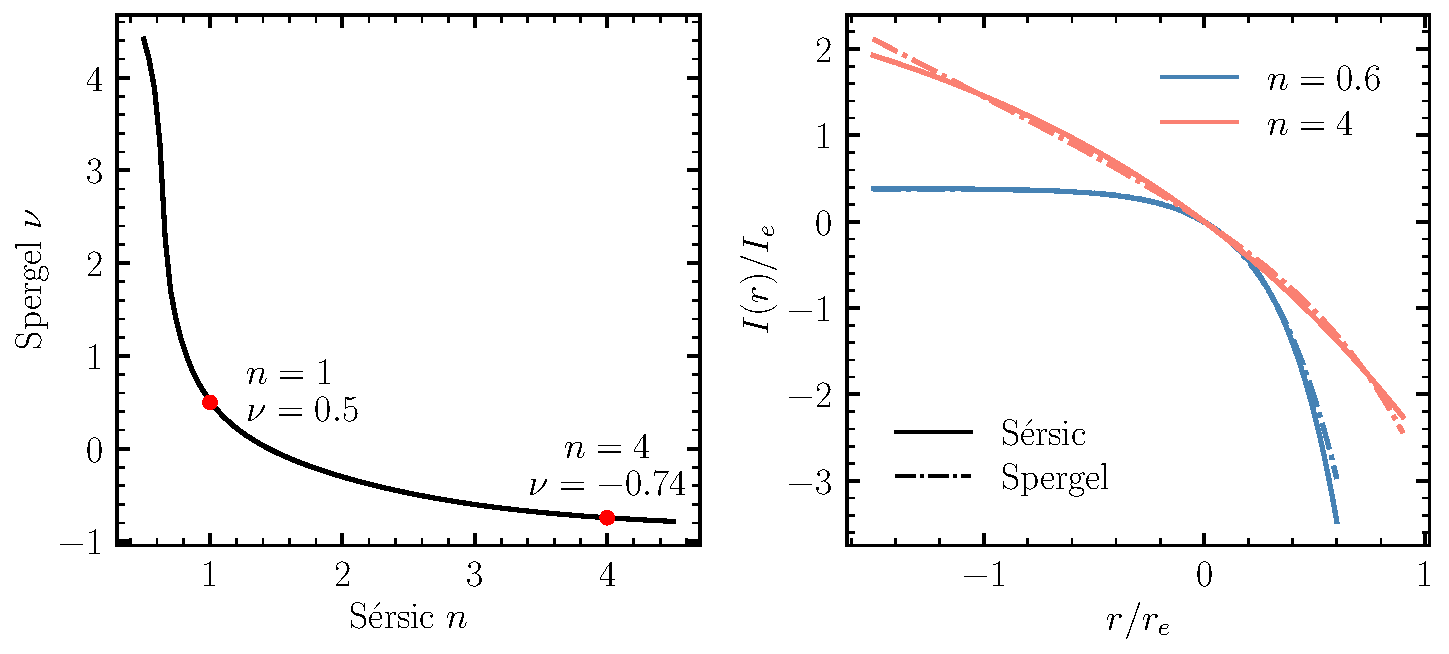
\includegraphics[width=0.75\linewidth]{spergel_sersic_calib.pdf}
	}
    \caption{The correspondence between the \sersic{} profile \eqref{eq:sersic} and the Spergel profile \eqref{eq:spergel}. We fit a Spergel profile to \sersic{} while fixing the total luminosity and half-light radius. The left panel shows the best-fit Spergel index $\nu$ as a function of \sersic{} index $n$. In the right panel, two \sersic{} profiles (solid) and their best-fit Spergel profiles (dash-dotted) are shown. Spergel profile approximates \sersic{} well for small \sersic{} indices.  
    }
    \label{fig:spgl_calib}
\end{figure*}


\section{Measurement Error}\label{ap:meas_error}

We characterize the quality of the Spergel modeling by injecting mock \sersic{} galaxies into the cutout and compare the recovered properties with the truth, as shown in Appendix \ref{ap:meas_error}. Overall speaking, the measurement agrees with the truth quite well. However, the size and the total flux of galaxies below $\overline{\mu}_{\rm eff} (g) > 27$ is under-estiamted. We also characterize the bias and the scatter in measurement as a function of size and surface brightness. We apply the bias correction to the measurement of LSBGs, and incorporate the measurement error into the science figures. 



vdB 16 doesn't consider whether GALFIT gives the corrrect $R_e$, when deriving the completeness (recovered fraction)

Remember to ref SMUDGES papers here.


\section{Catalog}
\onecolumngrid 

\begin{table}
\caption{UDG (UPG) catalog description} 
\label{tab:catalog}
\begin{center}
\begin{tabular}{l l l}
\hline\hline
% \multicolumn{3}{c}{Table: LSBGs (781 rows)}                 \\
% \hline
Column Name      & Unit    & Description                    \\
\hline
ID                       &         & Unique LSBG ID \\
ra                       & deg     & Right ascension (J2000) \\
dec                      & deg     & Declination (J2000) \\
$r_e$         & arcsec  & Circularized effective radius  \\
$\sigma(r_e)$ & arcsec  & Uncertainty of $r_e$ \\
$\overline{\mu}_{\mathrm{eff}}(g)$               & \sbunit & $g$-band average surface brightness within $r_e$ \\
$\sigma(\overline{\mu}_{\mathrm{eff}}(g))$       & \sbunit & Uncertainty of $\overline{\mu}_{\mathrm{eff}}(g)$           \\
$\overline{\mu}_{\mathrm{eff}}(r)$               & \sbunit & $r$-band average surface brightness within $r_e$ \\
$\sigma(\overline{\mu}_{\mathrm{eff}}(r))$       & \sbunit & Uncertainty of $\overline{\mu}_{\mathrm{eff}}(r)$           \\
$\overline{\mu}_{\mathrm{eff}}(i)$               & \sbunit & $i$-band average surface brightness within $r_e$ \\
$\sigma(\overline{\mu}_{\mathrm{eff}}(i))$       & \sbunit & Uncertainty of $\overline{\mu}_{\mathrm{eff}}(i)$           \\
$m_g$                    & mag     & $g$-band apparent magnitude     \\
$\sigma(m_g)$            & mag     & Uncertainty of $m_g$            \\
$m_r$                    & mag     & $r$-band apparent magnitude     \\
$\sigma(m_r)$            & mag     & Uncertainty of $m_r$            \\
$m_i$                    & mag     & $i$-band apparent magnitude     \\
$\sigma(m_i)$            & mag     & Uncertainty of $m_i$            \\
$g-r$                    & mag     & $g-r$ color                     \\
$\sigma(g-r)$           & mag     & Uncertainty of $g-r$ color      \\
$g-i$                    & mag     & $g-i$ color                     \\
$\sigma(g-i)$           & mag     & Uncertainty of $g-i$ color      \\
$\nu$                    &         & Spergel index              \\
$\varepsilon$               &         & Ellipticity                     \\
$A_g$                    & mag     & $g$-band Galactic extinction \\
$A_r$                    & mag     & $r$-band Galactic extinction \\
$A_i$                    & mag     & $i$-band Galactic extinction \\
\hline\hline
\end{tabular}
\end{center}
\tablecomments{
These tables are published in their entirety in machine-readable format.
Magnitudes are on the AB system and have not been corrected for Galactic
extinction. We provide Galactic extinction corrections, which are derived from
the \citet{Schlafly2011} recalibration of the \citet{SFD1998} dust maps. 
}
\end{table}


\end{CJK*}
\end{document}